%Varaibl dependiente Diagnostico de cancer

\subsection{El Cáncer}
Según la página del Instituto nacional del cáncer esta enfermedad se caracteriza por la multiplicación de algunas células anormales o dañadas del cuerpo humano, que se dispersan a otras partes del organismo. Llegando a formar tumores. \parencite{cancer_2024 }
El origen de este puede atribuirse a errores en la división celular, factores hereditarios o influencias externas como el entorno y la exposición a sustancias químicas. El desarrollo del cáncer es único en cada individuo, ya que cada persona tiene combinaciones genéticas diferentes, lo que hace que el tratamiento no sea igual para todos los casos.

\begin{figure}[h]
	\begin{center}
		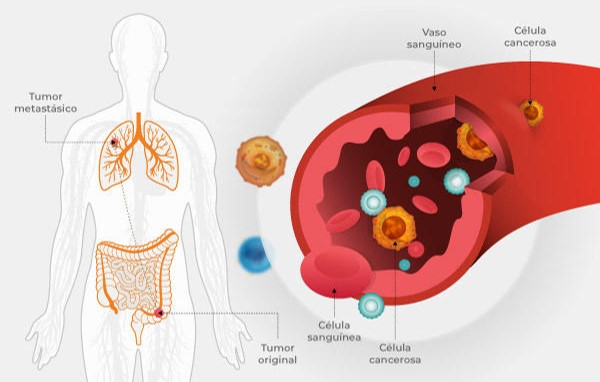
\includegraphics[width=0.6\textwidth]{2/figuras/imagenes/queeselcancer.jpg}
		\caption{Ejemplo como el cancer se traslada a otras partes del cuerpo. Fuente: \cite{cancer_2024}}
		\label{1:fig 15}
	\end{center}
\end{figure}


\subsection{Cáncer de Piel}
El cáncer de piel es el tipo de cáncer más prevalente a nivel mundial. Si bien algunas personas presentan un riesgo de contraerlo, puede afectar a cualquier persona. Este se origina a partir de la formación de células malignas en el tejido cutáneo.
Suele desarrollarse en áreas de la piel que están expuestas al sol; sin embargo, también puede aparecer en zonas que normalmente no están expuestas a la luz solar.
Las principales causas del cáncer de piel se deben a la exposición excesiva a los rayos UV del sol, así como al uso de camas bronceadoras y lámparas solares. Los rayos UV tienen la capacidad de dañar las células de la piel. A corto plazo, este daño puede resultar en quemaduras solares. Con el tiempo, la acumulación del daño por rayos UV provoca cambios en la textura de la piel, envejecimiento prematuro y, en ocasiones, cáncer de piel. \parencite{cancer_piel_clinic_2024}

\subsection{Sintomas del Cáncer de Piel}
Según la American Cancer Society, los médicos sugieren que los exámenes de la piel se incluyan en las revisiones médicas de rutina. De lo contrario, recomiendan que las personas examinen su propia piel aproximadamente una vez al mes. Este autoexamen debe realizarse frente a un espejo, en una habitación bien iluminada, para poder revisar cada área del cuerpo hasta las difíciles de ver. Es importante tener en cuenta la regla del "ABCDE" para identificar signos comunes de problemas en la piel: Asimetría, Borde, Color, Diámetro y Evolución. Estas pautas ayudan a detectar posibles irregularidades en la piel que podrían indicar la presencia de cáncer u otras afecciones.
\parencite{information_cancer}

\subsection{Factores de Riesgo}



\subsection{Tipos del Cáncer de Piel}
El cáncer de piel se clasifica en dos grandes categorías: cáncer de piel de tipo no melanoma y cáncer de piel de tipo melanoma. El cáncer de piel de tipo no melanoma se subdivide en carcinomas de células basales y carcinomas de células escamosas. Aunque generalmente son malignos, pueden curarse; sin embargo, si no se tratan a tiempo, pueden causar desfiguración y resultar muy costosos de tratar. Por otro lado, el cáncer de piel de tipo melanoma es responsable de la mayoría de las muertes relacionadas con el cáncer de piel, debido a su tendencia a propagarse a otras partes del cuerpo, incluidos los órganos vitales.

\subsection{Melanoma}
El melanoma, también conocido como melanoma maligno y melanoma cutáneo, se origina a partir de los melanocitos, las células especializadas de la piel encargadas de producir melanina. La melanina es responsable del tono bronceado o rojizo que adquiere la piel al exponerse al sol. Este tipo de cáncer tiene un gran potencial maligno, siendo responsable de más del 90\% de las muertes relacionadas con el cáncer de piel. Aunque el melanoma afecta principalmente a la piel, también puede desarrollarse en las mucosas y dentro del ojo. Generalmente, los melanomas se forman en la piel sana, pero en aproximadamente un 20-30\% de los casos, pueden desarrollarse sobre un lunar preexistente.  \parencite{cancer_tipo_melanoma}
Este comportamiento agresivo y su capacidad de propagarse rápidamente a otras partes del cuerpo, incluidos los órganos vitales, hacen que el melanoma sea especialmente peligroso y mortal, destacándose como una de las formas más graves de cáncer de piel.

\subsection{Formas de diagnosticar el cáncer de piel}
El primer paso en la detección de posibles problemas en la piel es realizar un examen con un médico especialista o alguien con conocimiento en el área. Durante este examen, se busca identificar cualquier lesión nueva o inusual. Si se encuentra alguna, el médico evaluará la lesión utilizando herramientas como el dermatoscopio, la dermatoscopia digital, la microscopía de reflectancia confocal o la ecografía cutánea. Sin embargo, para confirmar el diagnóstico, siempre es necesario realizar una biopsia de piel para su análisis en el laboratorio. Este procedimiento es actualmente la única manera de determinar con certeza si una persona tiene cáncer de piel y, en caso sea afirmativo, identificar el tipo específico de cáncer presente. \parencite{clinica_barcelona}


%\subsection{Detección Temprana}